\chapter{Notice de montage}
Le montage de la machine se fait grâce aux 7 étapes suivantes:

\begin{enumerate}
    \item Montage des réservoirs finaux
    \item Montage des cylindres perforés sur l'axe du distributeur
    \item Montage des goupilles et des roulements dans les parois gauches et droites
    \item Montage du distributeur et du couvercle sur la paroi gauche
    \item Montage des composantes centrales
    \item Montage de la paroi droite et la manivelle
    \item Montage des plaques du fond
\end{enumerate}

\newpage

\begin{enumerate}

\begin{figure}
    \centering
    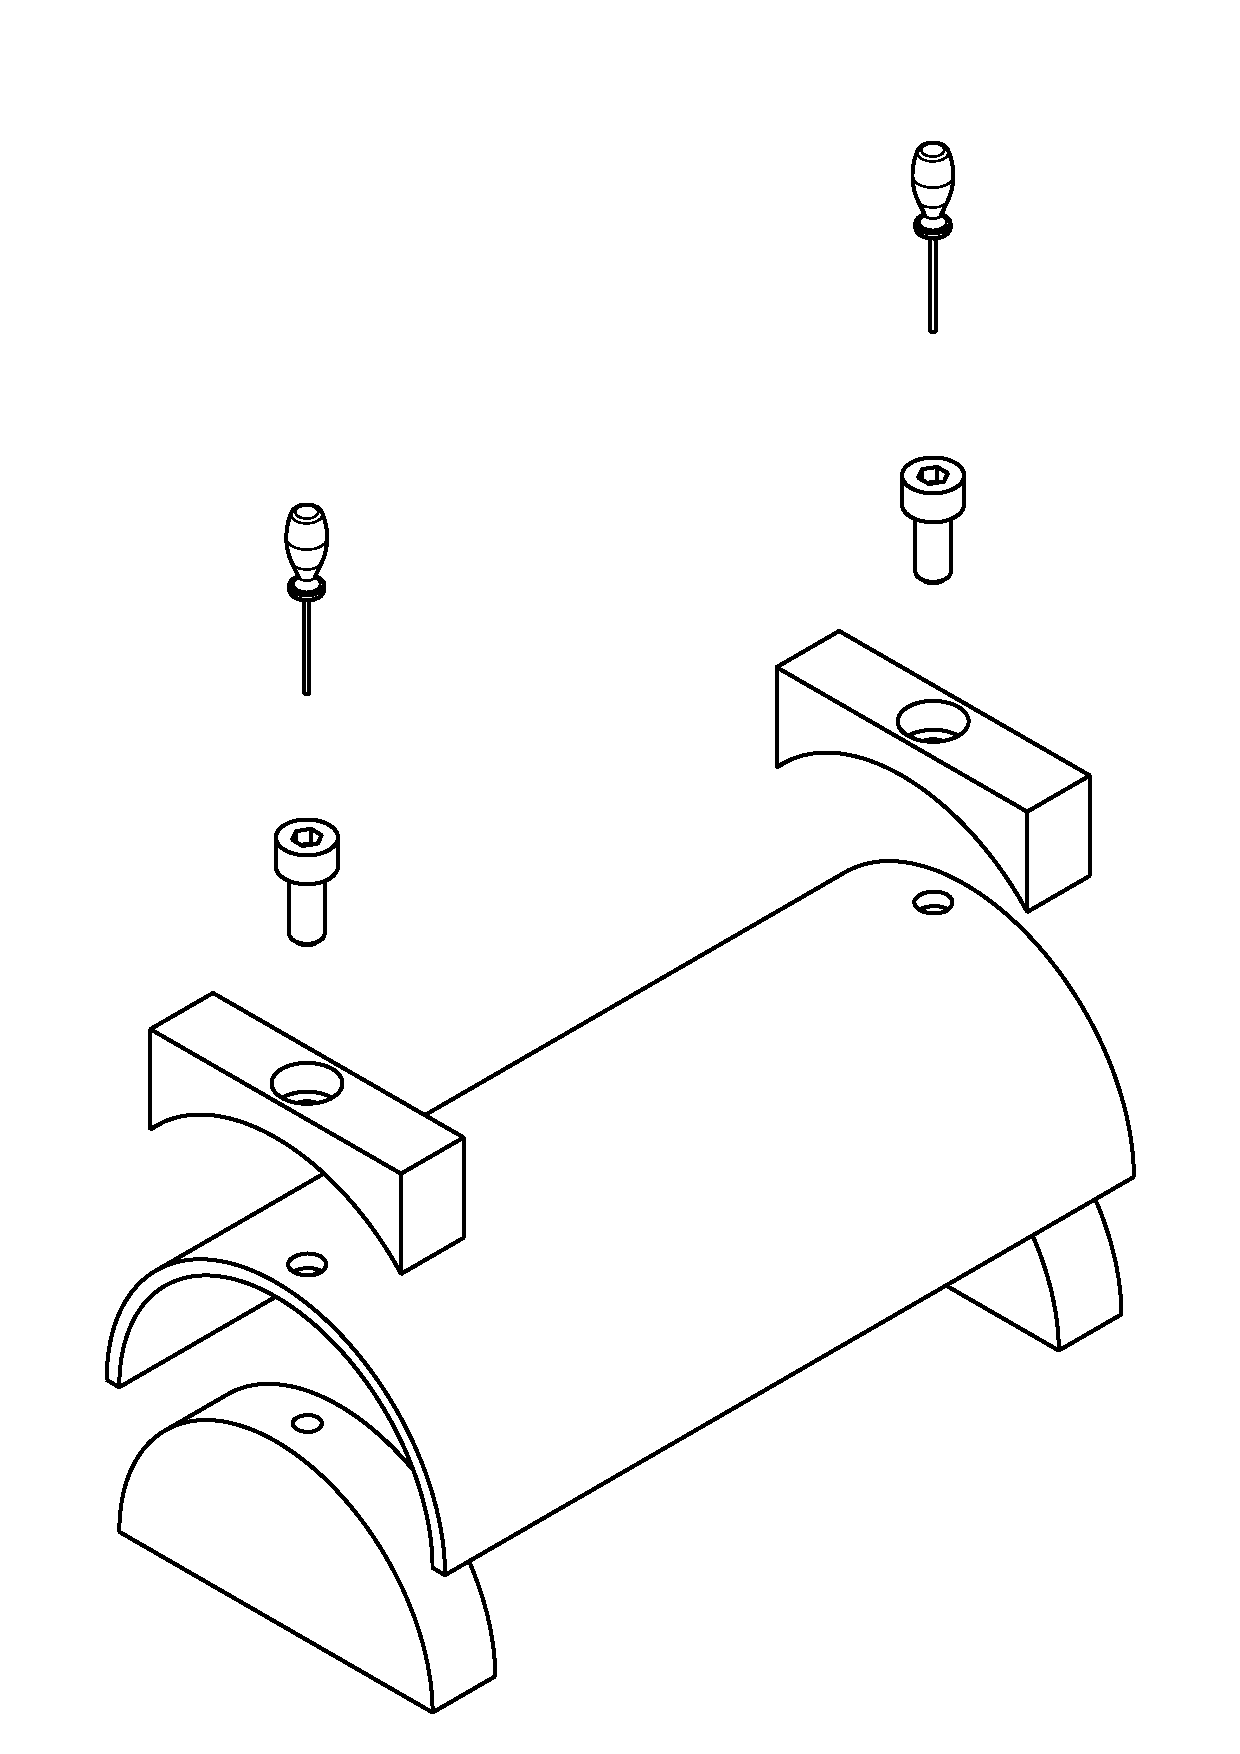
\includegraphics[width=0.65\textwidth]{Graphics/Montage/1.pdf}
    \caption{Montage 1}
    \label{fig:Montage1}
\end{figure}

\item A l'aide d'une clé allen de 3, assembler deux bords réservoir pour billes triées (pièces \No6), un tube réservoir pour billes triées (pièce \No7), deux pieds réservoir pour billes triées (pièce \No5), avec deux vis M4x10 (pièce \No20). %piece 21 n'existe plus /:

\newpage

\begin{figure}
    \centering
    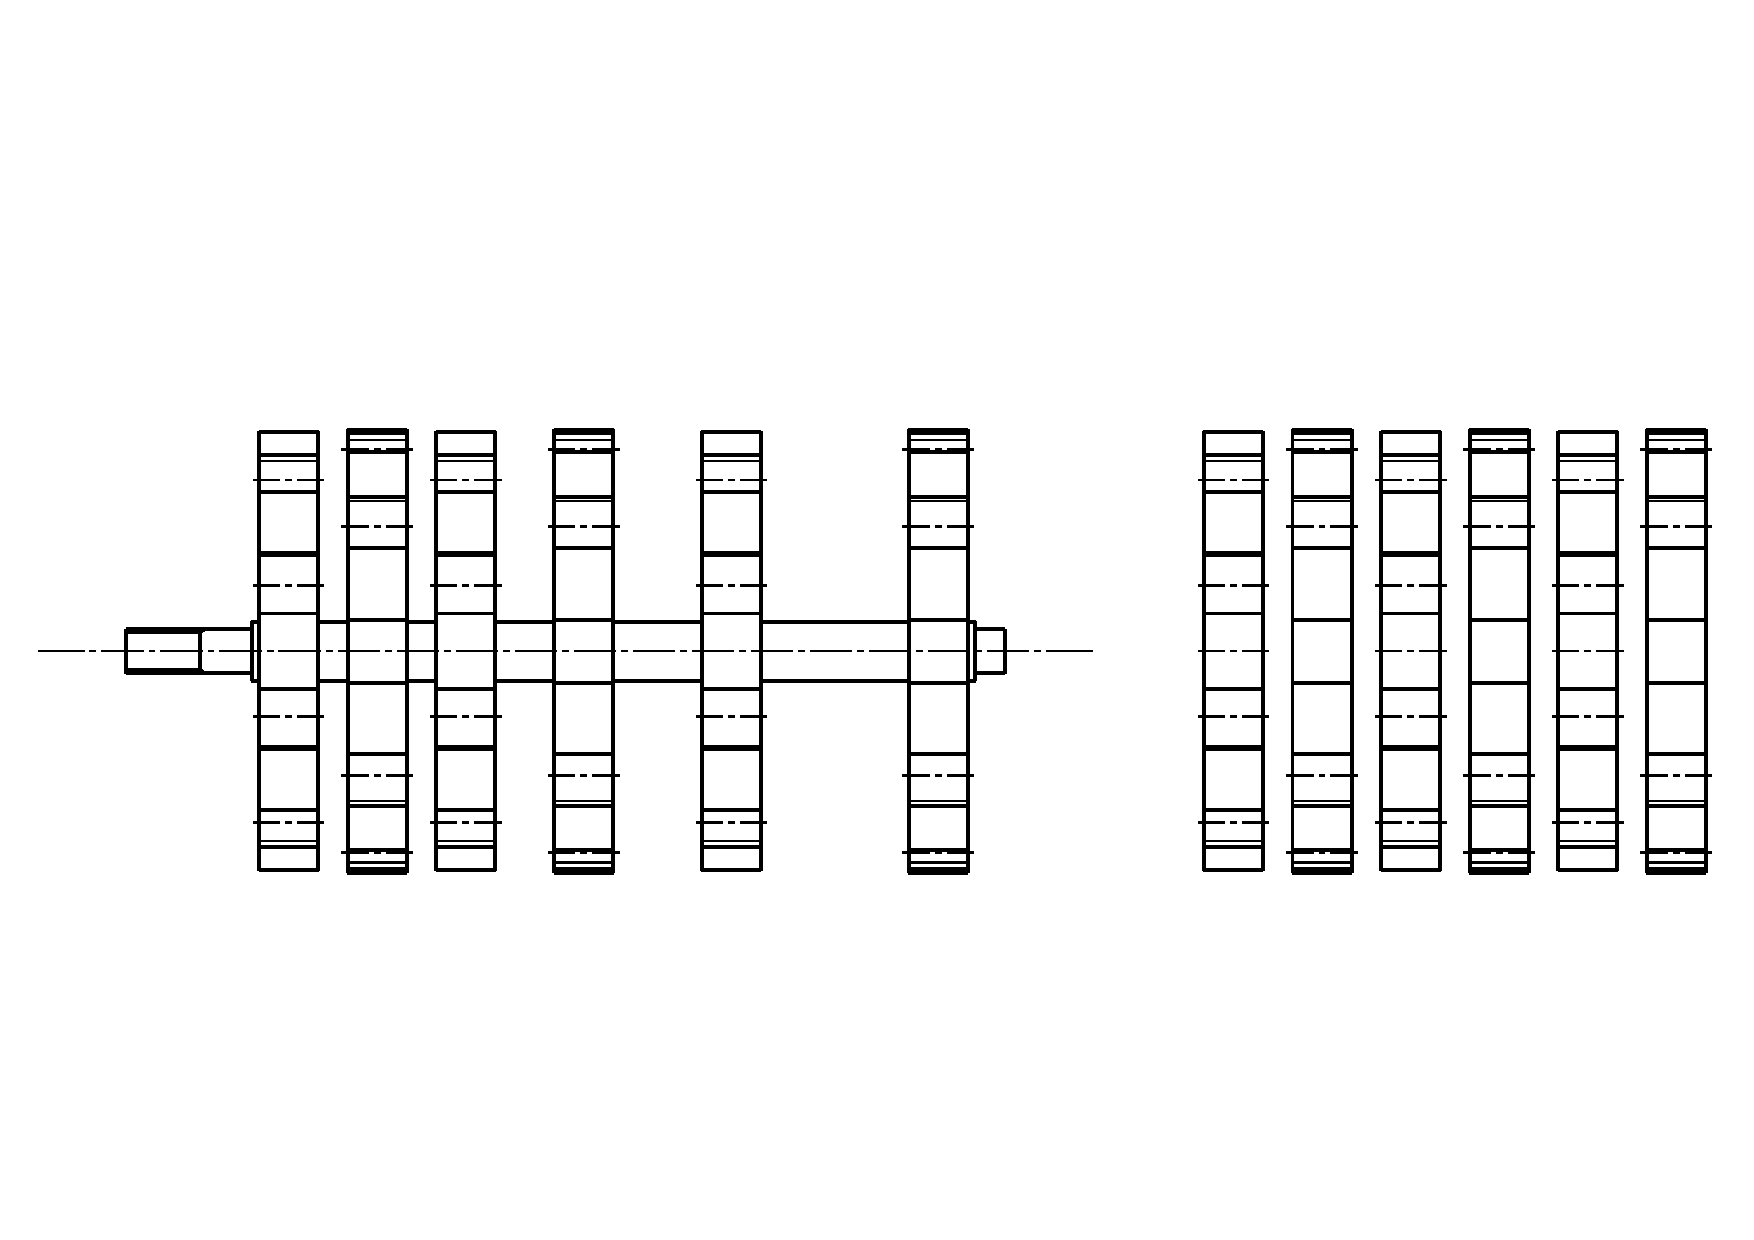
\includegraphics[width=\textwidth]{Graphics/Montage/2.pdf}
    \caption{Montage 2}
    \label{fig:Montage2}
\end{figure}

\item  Chauffer les cylindres perforés (pièce \No14) jusqu'à une température de \SI{275}{\degreeCelsius}, avant de les chasser sur l'axe du distributeur (pièce \No13). Les cylindres sont ainsi assemblés par serrage sur l'axe.

\newpage

\begin{figure}
    \centering
    \begin{subfigure}[h]{0.45\linewidth}
        \centerfloat
        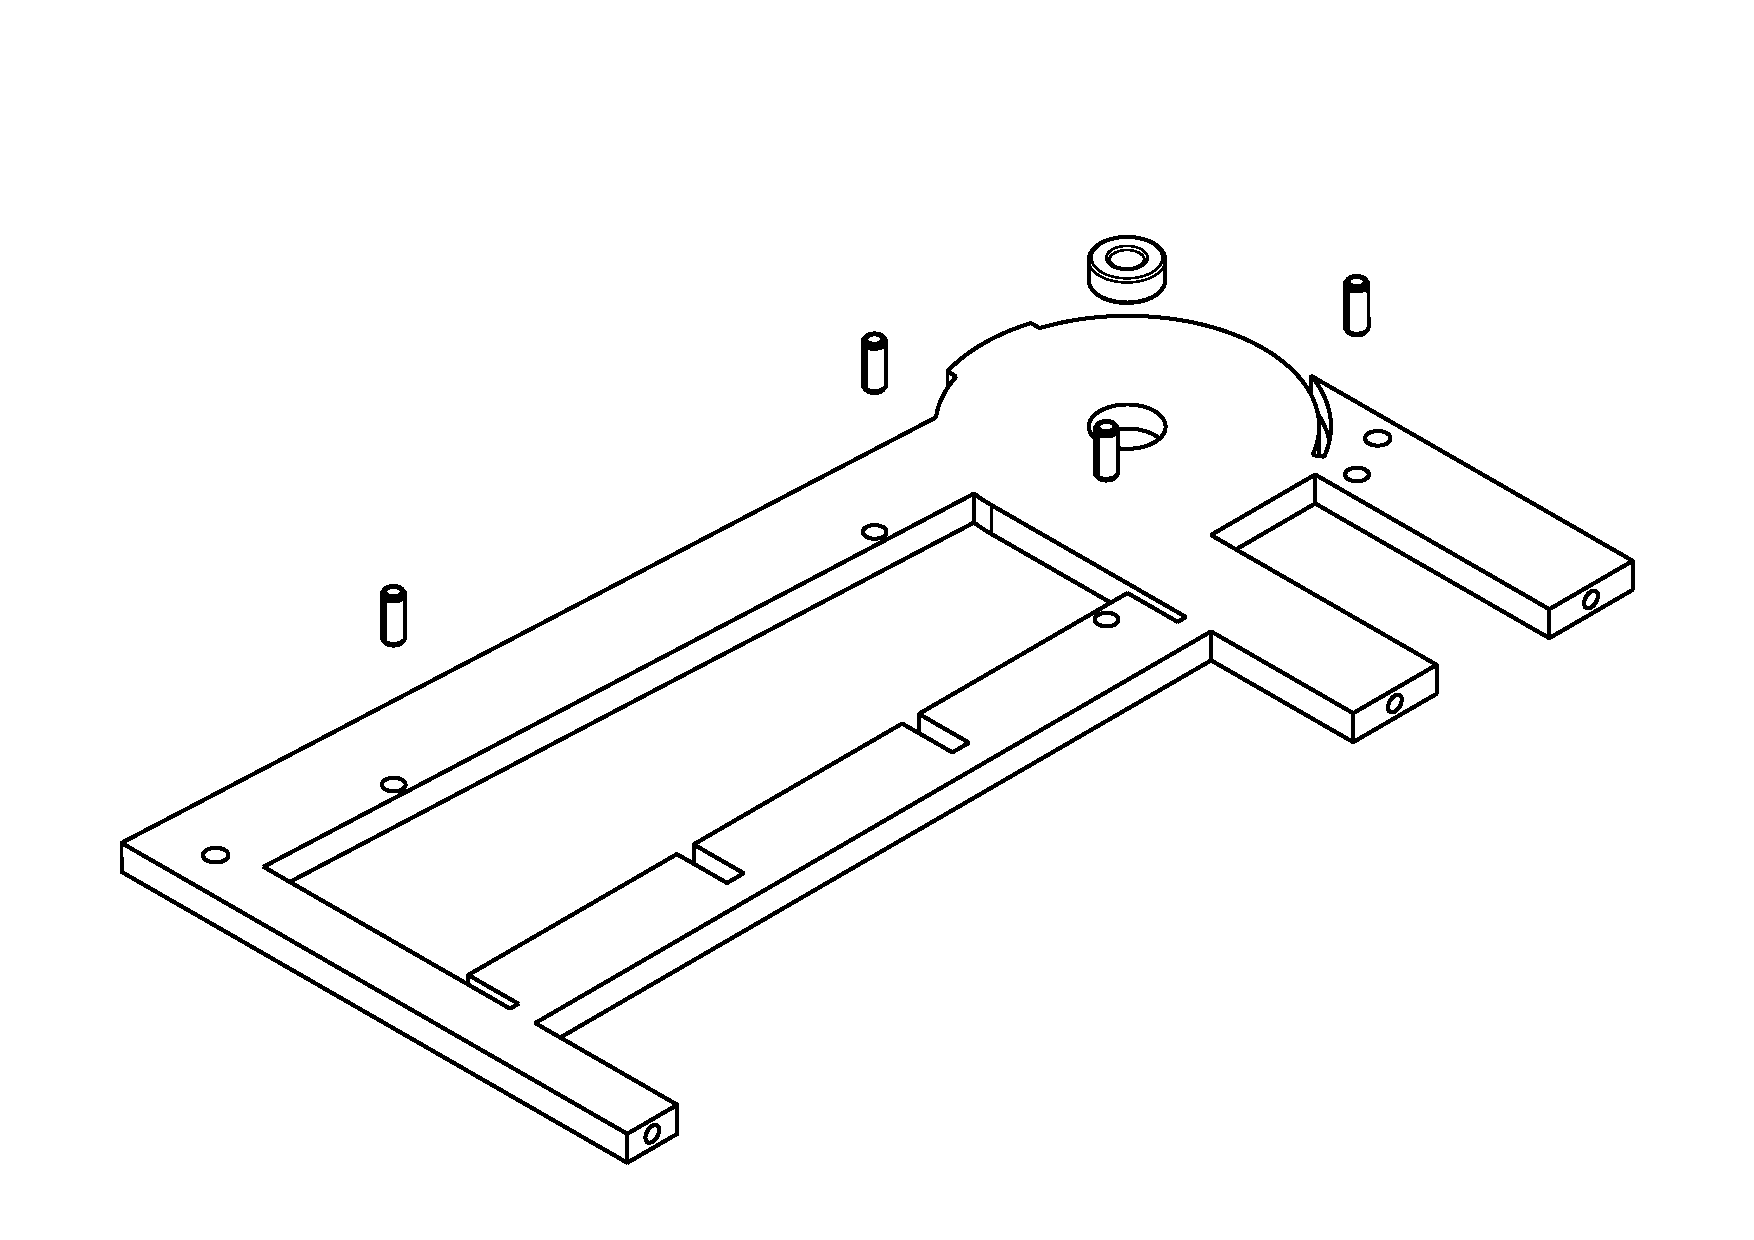
\includegraphics[width=1.25\linewidth]{Graphics/Montage/3A.pdf}
    \end{subfigure}
    \hfill
    \begin{subfigure}[h]{0.45\linewidth}
        \centerfloat
        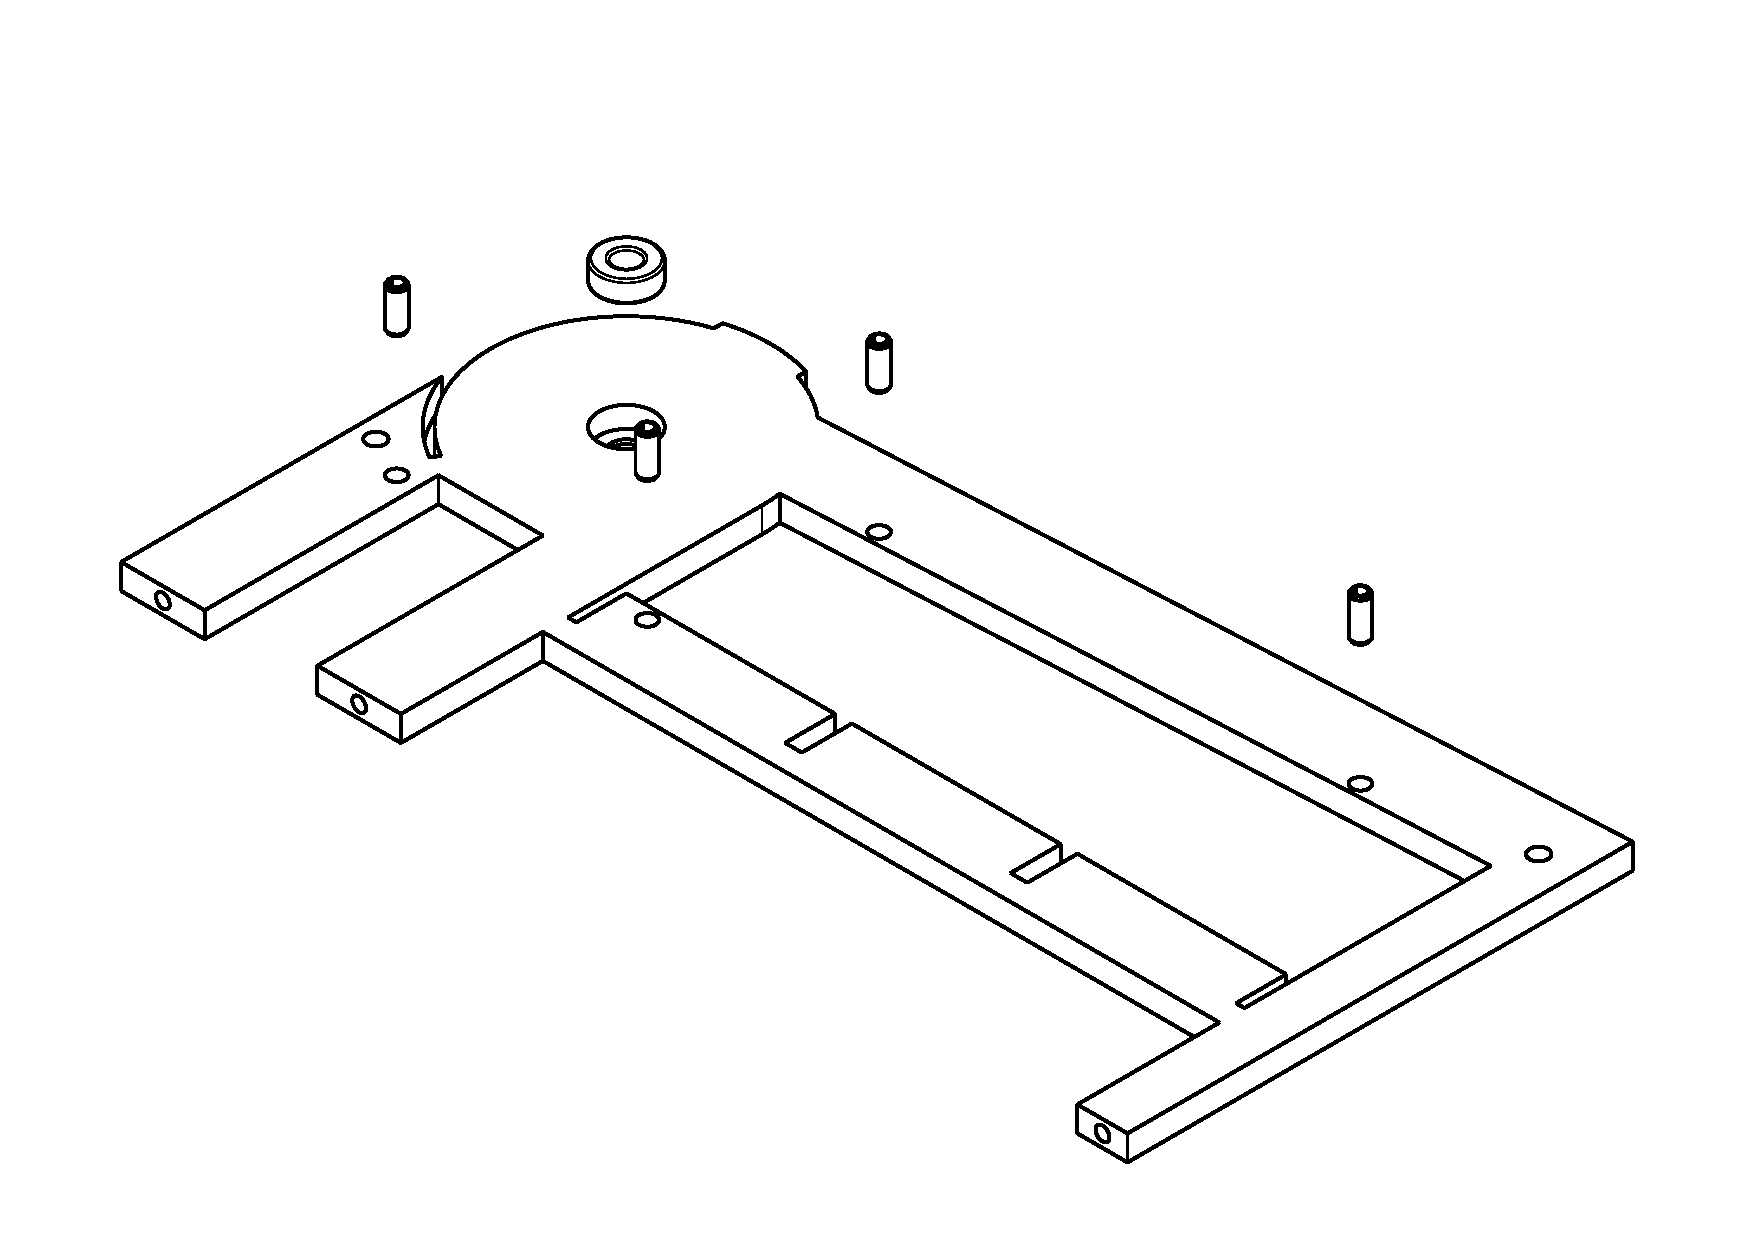
\includegraphics[width=1.25\linewidth]{Graphics/Montage/3B.pdf}
    \end{subfigure}
    \caption{Montage 3}
    \label{fig:Montage3}
\end{figure}

\item Chasser les goupilles (pièce \No18) dans leurs logements sur les pièces fixation gauche (pièce \No4) et fixation droite (pièce \No3). Chasser les roulements à bille (pièce \No17) dans les trous de diamètre \SI{7}{\mm} des deux pièces fixation.

\newpage

\begin{figure}
    \centering
    \centerfloat
    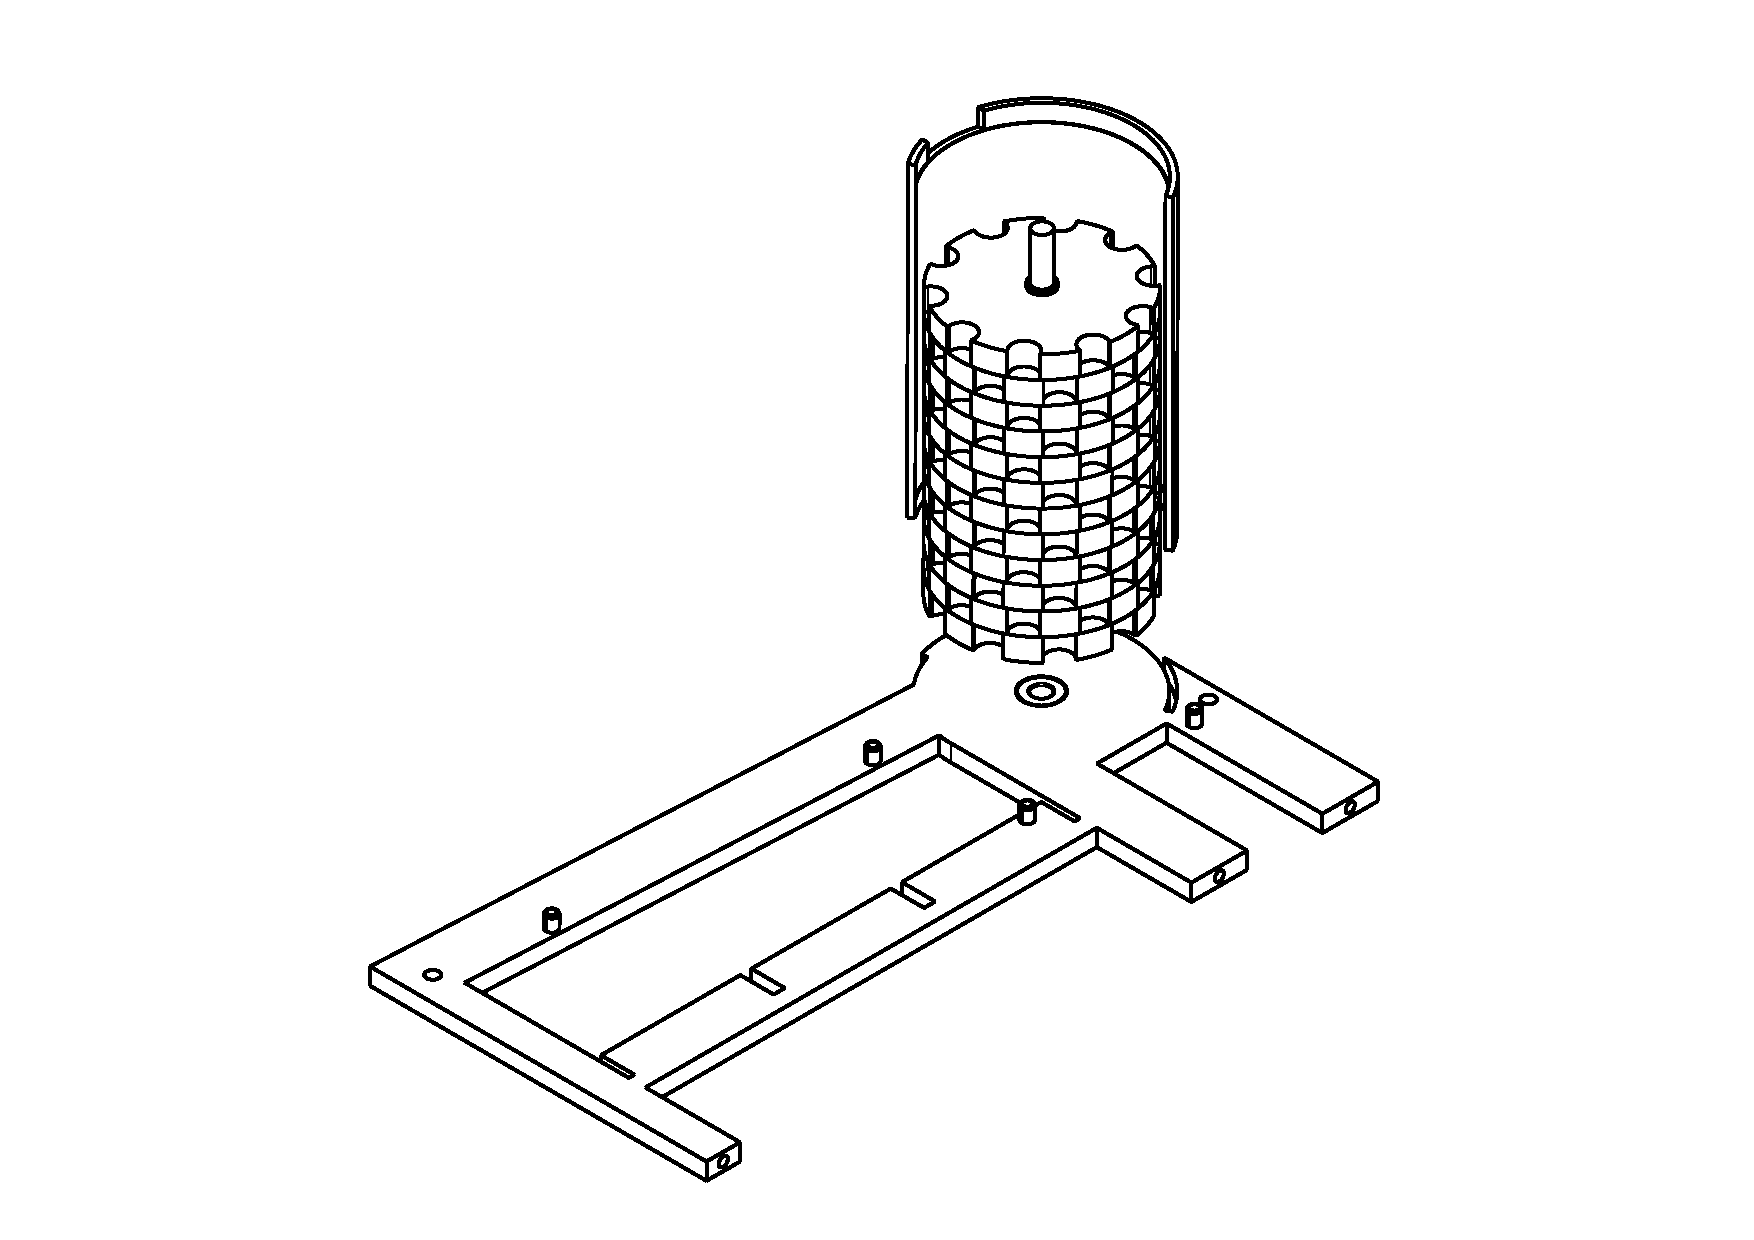
\includegraphics[width=1.3\textwidth]{Graphics/Montage/4.pdf}
    \caption{Montage 4}
    \label{fig:Montage4}
\end{figure}

\item Monter l'axe et les cylindres ainsi que le cache (pièce \No15) sur la pièce fixation gauche.

\newpage

\begin{figure}
    \centering
    \centerfloat
    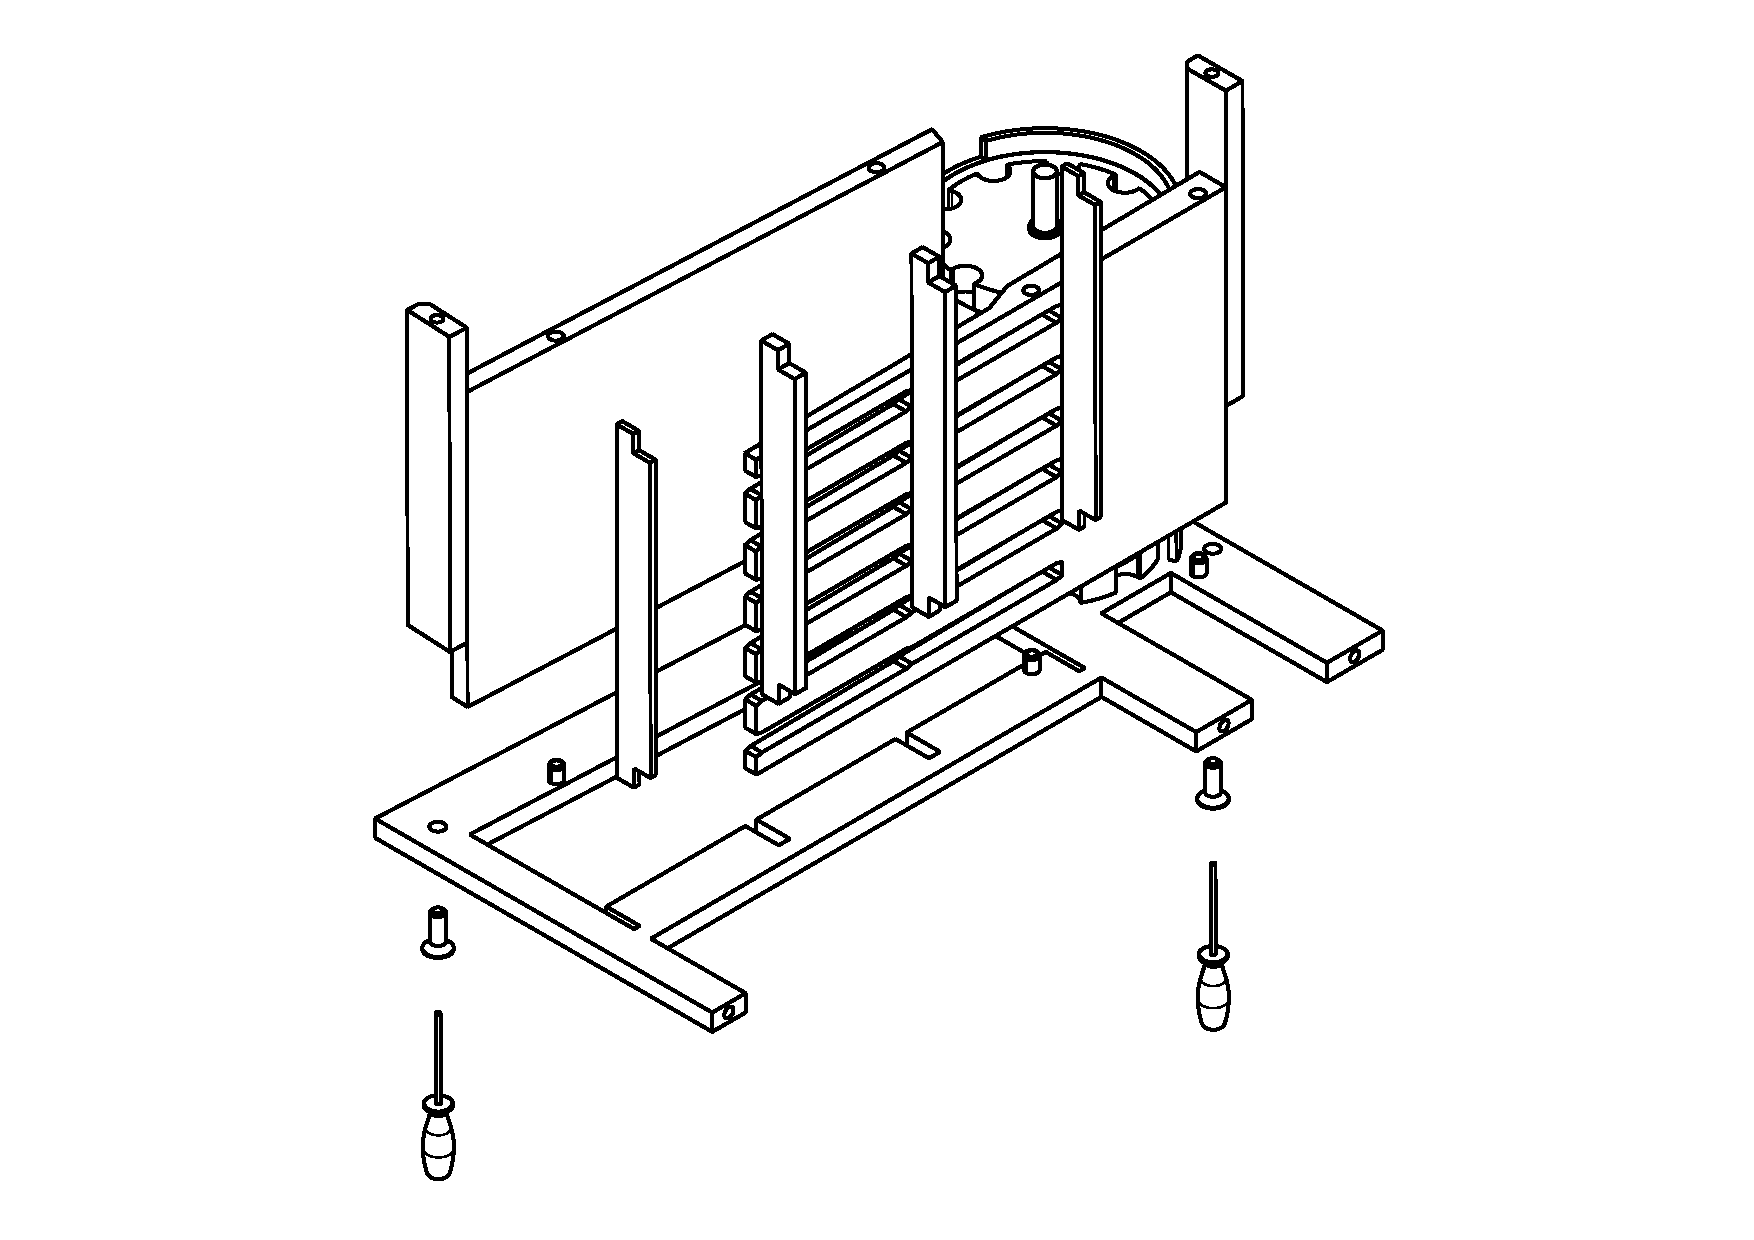
\includegraphics[width=1.3\textwidth]{Graphics/Montage/5.pdf}
    \caption{Montage 5}
    \label{fig:Montage5}
\end{figure}

\item Chasser le fond réservoir pour billes mixtes (pièce \No12) sur la pièce fixation gauche, grâce aux goupilles. Assembler, à l'aide d'une clé allen de 2.5, le bord avant et le bord arrière (pièces \No11) avec la pièce fixation gauche, grâce à deux vis M4x12 (pièces \No19). Assembler ensuite les deux limitations épaisses (pièce \No8) et fines (pièce \No9) dans la pièce fixation gauche. Chasser finalement le séparateur (pièce \No10) sur les deux goupilles.

\newpage

\begin{figure}
    \centering
    \centerfloat
    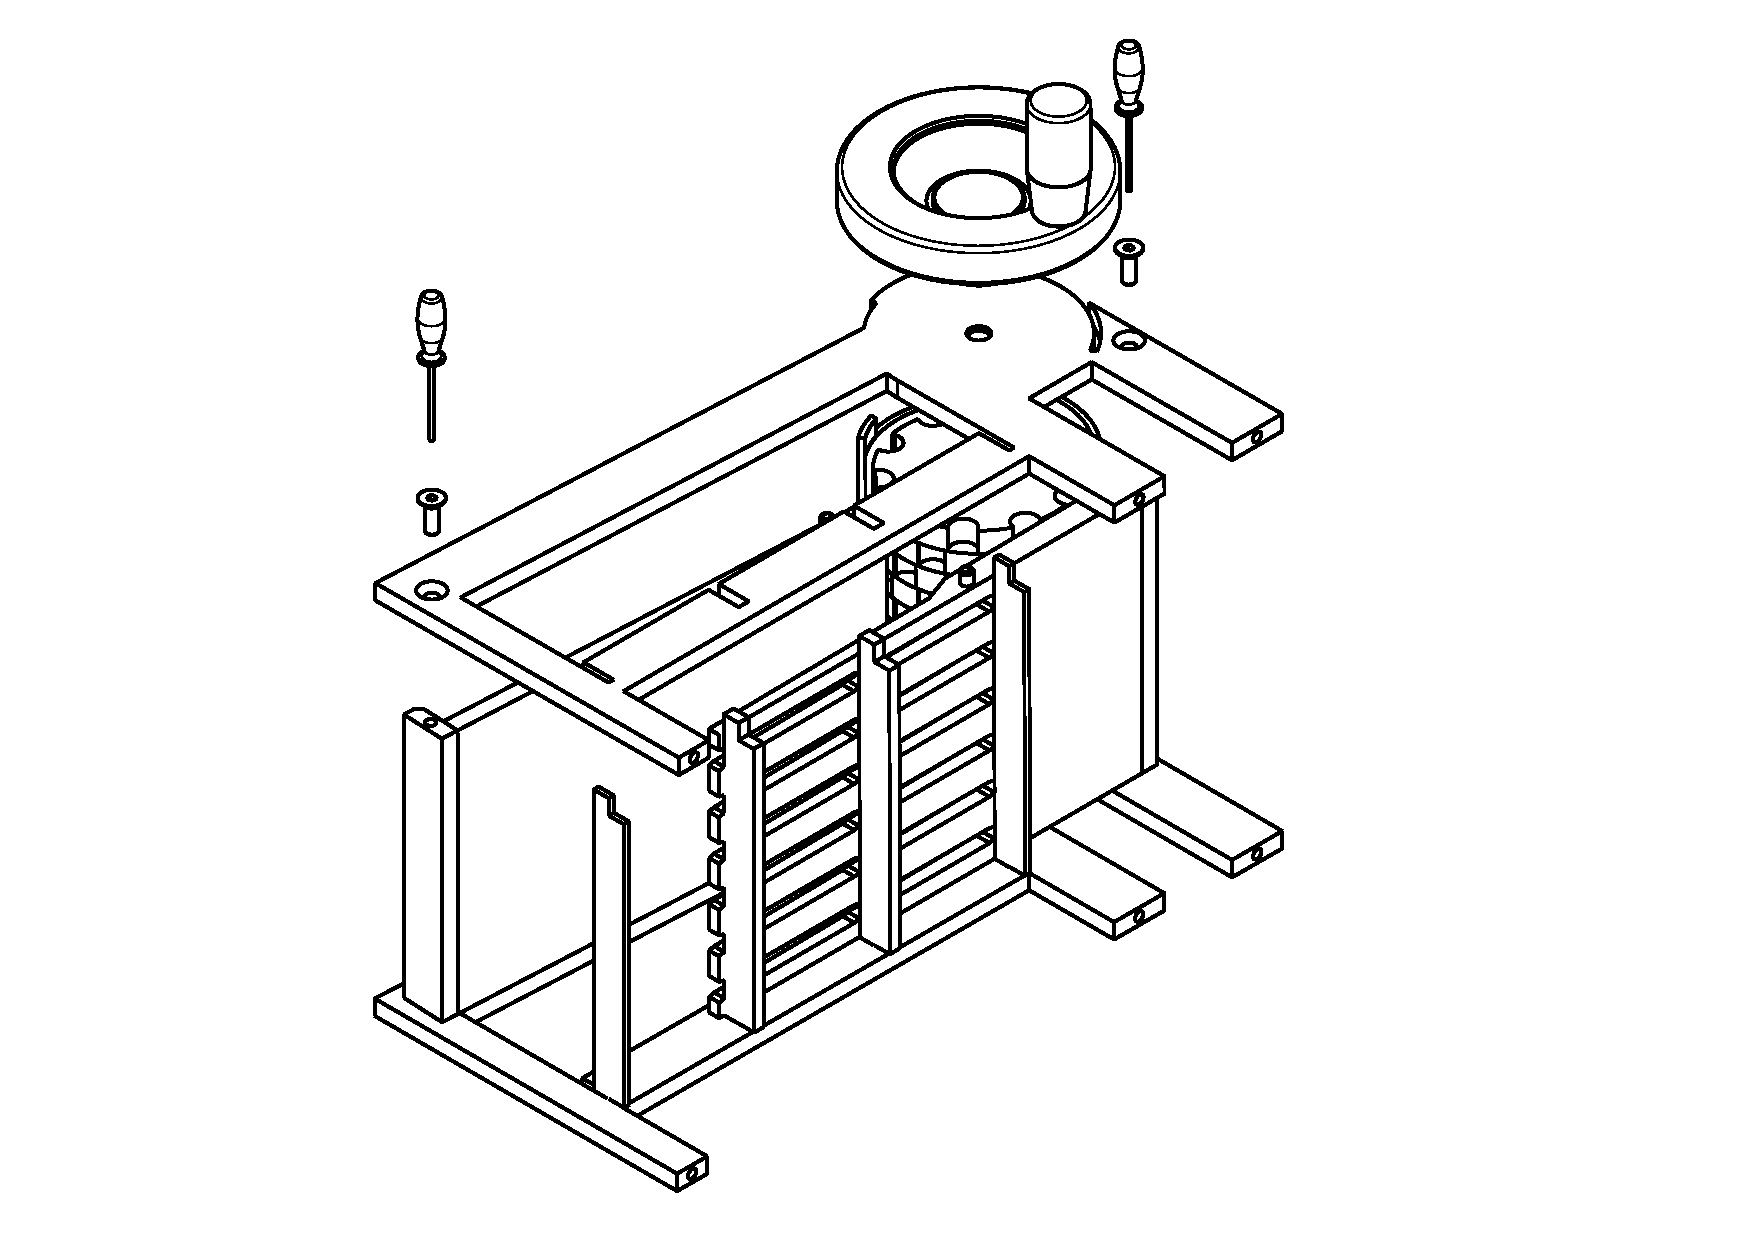
\includegraphics[width=1.35\textwidth]{Graphics/Montage/6.pdf}
    \caption{Montage 6}
    \label{fig:Montage6}
\end{figure}

\item A l'aide d'une clé allen de 2.5, assembler la pièce fixation droite sur l'ensemble construit jusqu'à présent, grâce à deux vis M4x12 (pièces \No19). Visser ensuite la manivelle (pièce \No16) sur le filetage de l'axe. 

\newpage

\begin{figure}
    \centering
    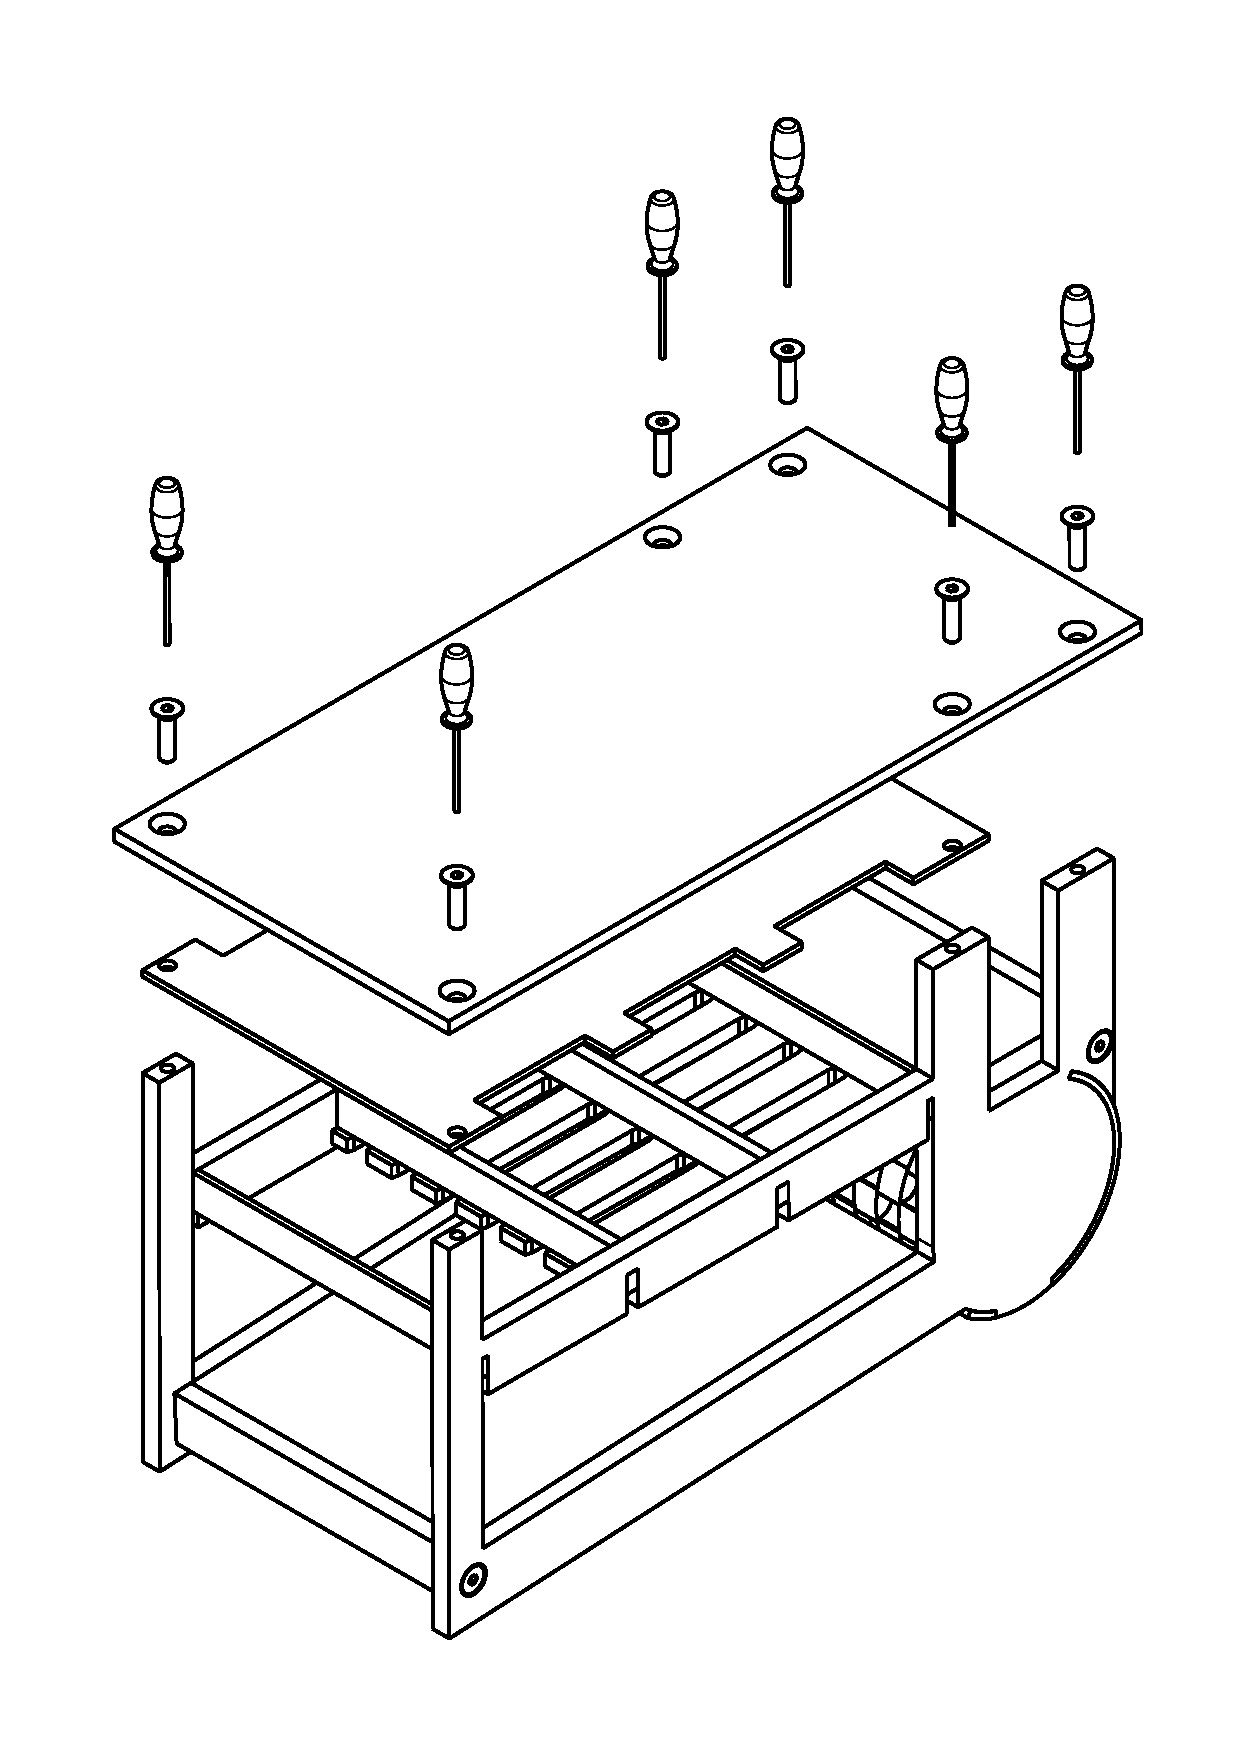
\includegraphics[width=0.65\textwidth]{Graphics/Montage/7.pdf}
    \caption{Montage 7}
    \label{fig:Montage7}
\end{figure}

\item Finalement, assembler la plaque de fond (pièce \No1) et la pièce fixation des réservoirs (pièce \No2) grâce à 6 vis M4x12 (pièces \No19).
%J'ai changé les vis M4x16 avec les M4x12 parce que les autres étaient trop long...

\end{enumerate}